\documentclass{article}


\usepackage{float}
\documentclass[a4paper]{article}
%%%%%%%%%%%%%%%%%%%%%%%%%%%%%%%%%%
% Package for making LaTeX properly handle utf8 characters set and danish language rules
\usepackage[utf8]{inputenc}
\usepackage[danish]{babel}
%%%%%%%%%%%%%%%%%%%%%%%%%%%%%%%%%%
% Package for changing to a nicer font 
\usepackage [T1]{fontenc}
%%%%%%%%%%%%%%%%%%%%%%%%%%%%%%%%%%
% Package for conctroling the text area
\usepackage[margin=2.5cm]{geometry}
%%%%%%%%%%%%%%%%%%%%%%%%%%%%%%%%%%
% Package for inserting clickable hyperlinks in pdf versions as produced by pdflatex
\usepackage{hyperref}
%%%%%%%%%%%%%%%%%%%%%%%%%%%%%%%%%%
% Package for including figures. TeX and thus LaTeX was developped before the existence of directory file-structures, but the graphicspath let's you add directories, that the \includegraphics will search.
\usepackage{graphicx}
\graphicspath{{figures/}{anotherFigureDirectory/}}
%%%%%%%%%%%%%%%%%%%%%%%%%%%%%%%%%%
% Package for typesetting programs. Listings does not support fsharp, but a little modification goes a long way
\usepackage{listings}
\usepackage{color}
\definecolor{bluekeywords}{rgb}{0.13,0.13,1}
\definecolor{greencomments}{rgb}{0,0.5,0}
\definecolor{turqusnumbers}{rgb}{0.17,0.57,0.69}
\definecolor{redstrings}{rgb}{0.5,0,0}
\lstdefinelanguage{FSharp}
                {morekeywords={let, new, match, with, rec, open, module, namespace,
type, of, member, and, for, in, do, begin, end, fun, function, try, mutable, if, 
then, else},
    keywordstyle=\color{bluekeywords},
    sensitive=false,
    morecomment=[l][\color{greencomments}]{///},
    morecomment=[l][\color{greencomments}]{//},
    morecomment=[s][\color{greencomments}]{{(*}{*)}},
    morestring=[b]",
    stringstyle=\color{redstrings}
    }
%%%%%%%%%%%%%%%%%%%%%%%%%%%%%%%%%%
% Package for extended math settings, e.g. \eqref
\usepackage{amsmath}
%%%%%%%%%%%%%%%%%%%%%%%%%%%%%%%%%%
\usepackage[utf8]{inputenc}

\title{Opgave 4g}
\author{Christer K. Lindholm, Carl-Emil Rohde og Emil Olesen }
\date{October 2022}

\begin{document}

\maketitle

\section*{4g0.}

\section*{Opsummering af problemformuleringer}


\section*{Løsningsmuligheder, overvejelser og argumenter}

\subsection*{4g0(a): Distance mellem source og target}
I den første delopgave, skal vi skrive en funktionen "dist: p1: pos -> p2: pos -> int", der givet to koordinatsæt - et startpunkt "source" og slutpunkt "target", udregner distancen mellem de to punkter. Til at gøre dette brugte vi formlen $distance = (x2 - x1)^2 - (y2 - y1)^2$.
Vores funktion "dist" tager to argumenter i form af tupler med koordinatsæt, hvor første og andenkoordnaterne identificeres ved brug af "fst" og "snd" kommandoen, bliver sat ind i formlen. For at funktionen vil udregne distancen, bliver vi nødt til at omregne fra heltal til kommatal. Dette gør vi ved, at "støbe" regnestykkerne i parantes med kommandoen "float"-nøgleordet. Funktionen fra opgaven påskriver dog, at funktionen returnerer heltal. Derfor som det sidste før vi printer resultatet, støber vi typen tilbage til heltal med "int()". 



\subsection*{4g0(b): Tættere på target, med candidate}
Vi skal i denne opgave skrive et program med typerne \emph{candidates: src: pos -> tg: pos -> pos list} til at bringe robotten tættere på target. I denne programmeringsdel tager vi fortsat udgangpunkt i \emph{source} og \emph{target} som værende henholdvis $(3,3)$ og $(1,1)$. Vores tankegang er, at lægge 1 til og trække 1 fra koordinaterne på \emph{source} for at få vores næste \emph{candidate}. Efterfølgende vil vi bruge \emph{List.filter} med en anonym funktion til, at vise den/de lister, der har mindre eller samme afstand til target, som afstanden mellem source og target. Resultatet ser ud som følgende. 
\begin{figure}[H]
    \centering
    
\includegraphics{Skærmbillede 2022-10-08 kl. 16.19.56.png}
    \caption{}
    \label{fig:my_label}
\end{figure}

Vi kan her se, at vi får to mulige udfald, der begge vil bringe os tættere på \emph{target}.

\vspace{20mm}
\subsection*{4g0(c): Samtlige korteste ruter til target}
Vi skal i denne opgave bygge et program, der fortæller brugeren samtlige muligheder for at komme fra \emph{source} til \emph{target} på den kortest mulige måde. Vi skal anvende programmeringsstrukturen: \emph{routes: src: pos -> tg: pos -> pos list list} - hvor en funktion, \emph{routes} der som input tager to positioner der henholdsvis er vores \emph{source} og \emph{target}, for at returnere positioner som lister i en liste. Det vil sige at, \emph{routes} skal returnere step by step, alle de ruter man kan benytte, for hurtigst at komme til \emph{target}.

Vi har lavet en rekursiv funktion, der bruger \emph{match with} til returnere en liste i en liste, når kordinaterne i listen $=$ \emph{target}. For alle andre udfald skal den bruge List.concat samt List.map, til at gennemgå alle andre muligheder, samt sortere alle ruter fra, der er længere end de korteste. Eftersom der findes flere måder hvorpå man kan bevæge sig fra a til b, og stadig have tilbagelagt samme afstand, vil programmet returnere flere anvendelige ruter, der stadig opfylde kriteriet for hurtigste rute. Man kunne forestille sig, at havde afstanden mellem \emph{source} og \emph{target} været tilpas stor, ville mulighederne tinærme sig et voldsomt stort tal, eftersom kombinationerne ville være mange.

\begin{figure}[H]
    \centering
    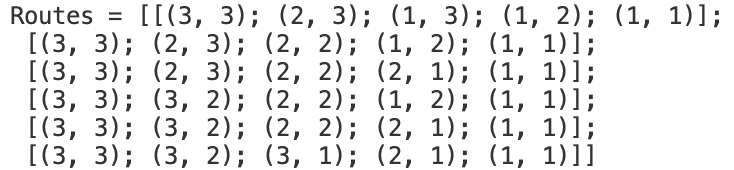
\includegraphics[scale=0.7]{Skærmbillede 2022-10-08 kl. 17.05.56.png}
    \caption{}
    \label{fig:my_label}
\end{figure}

Vi kan her se de korteste ruter fra \emph{source} til \emph{target}, angivet som tuples i lister, i en liste.



\subsection*{4g0(d): Korteste ruter med diagonale veje}
I denne opgave skal funktionen \emph{candidates} gøres i stand til også at bruge diagonale koordinater som bevægelser mod målet, mens \emph{routes} kun skal returnere de korteste ruter. 

\emph{Candidates} var allerede bygget til at gennemgå lister af mulige bevægelser samt til at filtrere dem fra, som ikke går tættere på target. For at indføre diagonale muligheder tilføjede vi blot nye lister til rækken af lister, den vurderer. Diagonale bevægelser svarer til lægge 1 til eller trække en fra i både første- og andenkoordinat samtidigt.

\emph{Routes} begynder nu at returnere et dramatisk øget antal mulige stier mod target. For at begrænse outputtet til de korteste, brugte vi listemodulets indbyggede funktioner:
\begin{enumerate}
    \item Vi binder den sammensatte liste af alle de mulige ruter fra \emph{routes} til navnet \emph{cons}.
    
    \item List.map funktionen løber igennem \emph{cons} og bruger List.length på hvert element. Den danner dermed en liste med antallet af bevægelser (tupler) i hver sti til målet.
    
    \item På listen med antallet af bevægelser, finder vi de korteste med List.min.
    
    \item Endelig kan List.filter løbe den originale \emph{routes}-liste igennem, mens den læser hver listes længde med List.length samt sortere alle lister fra, der ikke lig længden på den korteste stis liste.
\end{enumerate}
\begin{verbatim}
    let rec routes (src: pos) (tg: pos) : pos list list =
    match src with 
        p when p = tg -> [[tg]]   
        | _ -> 
            let allRoutes = List.map (fun elm -> 
                            List.map (fun elm2 -> src::elm2) (routes elm tg)) (candidates src tg)
            let cons = List.concat allRoutes 
            let mapList = List.map (fun list -> List.length list) (cons)
            let minimum = List.min mapList
            let filter = List.filter (fun elm -> List.length elm = minimum) (cons)
            filter 
\end{verbatim}


\end{document}
